\begin{frame}
    \frametitle{Conclusiones}

        \begin{block}{Cumplimiento de objetivos}
            \begin{itemize}
                \item Todos los objetivos marcados al inicio del PFC han sido cumplidos.
                \item Más duración de la esperada
                \item Contribución al mundo del software libre
                \item Juego de coches en 2D totalmente funcional
            \end{itemize}
        \end{block}

        \begin{block}{Valoración personal}
            \begin{itemize}
                \item Enfrentamiento a un proyecto complejo en solitario
                \item Aprendizaje de nuevas herramientas
                \item Puesta en práctica de conocimientos adquiridos
            \end{itemize}
        \end{block}


        \begin{block}{Posibles mejoras y ampliaciones:}
            \begin{itemize}
                \item \textbf{Modo dos jugadores}: pantalla dividida en dos.

                \item \textbf{Modo en red}: más conveniente que el modo de dos jugadores.
                
                \item \textbf{Varias resoluciones}: el usuario elige el tamaño mas cómodo.
                %cómodo para personas con pantalla muy pequeñas, como usuarios de netbooks, o también para persona con grandes resoluciones que desean una ventana de juego mayor.
                
                \item \textbf{Grabación de las mejores vueltas}: visualizarlas posteriormente.
                
            \end{itemize}
        \end{block}
        
\end{frame}

\begin{frame}
    \frametitle{Conclusiones}
    \begin{center}
        {\huge Zycars se incluirá en la próxima versión de}\\
        \begin{center}
            {\Huge Guadalinex}
        \end{center}
    \end{center}

        
    \begin{columns}
    
        \column{100px}
        \begin{center}
            
\includegraphics[scale=0.4]{imagenes/andatuz.png}
        \end{center}
        
        \column{200px}
        \begin{center}
            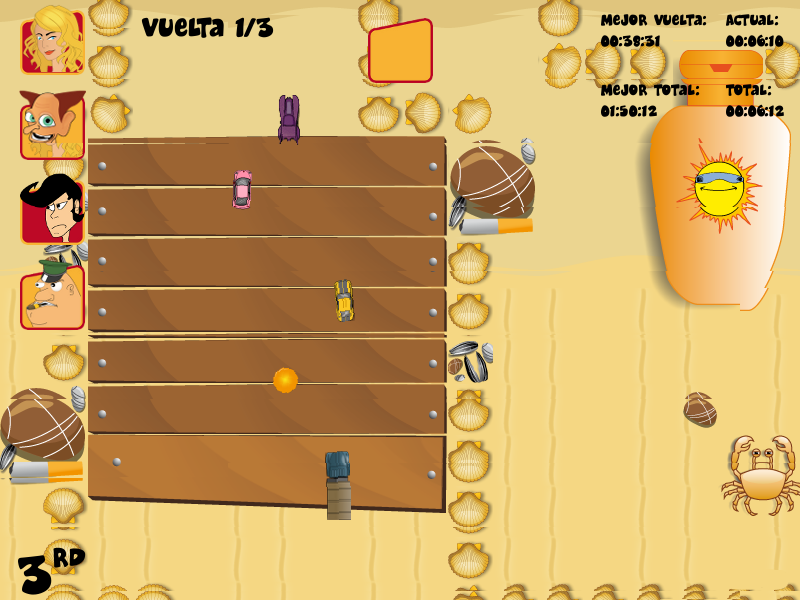
\includegraphics[scale=0.22]{imagenes/pantalla_juego.png}
        \end{center}
    \end{columns}

\end{frame}

